
\centerline{\textbf{ \LARGE Micro Programming, Micro instructions, RISC, CISC}}


\begin{questyle}
  \question  A micro instruction into be designed to specify \\ a). none or one of the three micro
             operations of one kind and \\b). none or upto six micro operations of another kind.
             The minimum number of bits in the micro-instruction is  (GATE-1997)

  \begin{oneparchoices}
    \choice         9
    \choice         5
    \CorrectChoice  8
    \choice         None
  \end{oneparchoices}
  \\ Hint : Micro-instruction specifies 7 micro-operations. (M0, M1, M2, M3, M4, M5, M6)
  \\ Hint : M0 has 3 types.
  \\ Hint : 2 bits : Only one from (M01, M02, M03, none)
  \\ Hint : 6 bits : Any combination from (M1, M2, M3, M4, M5, M6)

    \begin{myTableStyle} \begin{tabular}{ |m{1cm}|m{0.2cm}|m{0.2cm}|m{0.2cm}|m{0.2cm}|m{0.2cm}|m{0.2cm}|m{0.2cm}| } \hline
                & M0 & M1 & M2 & M3 & M4 & M5 & M6 \\ \hline
        Options & 4  & 2  & 2  & 2  & 2  & 2  & 2 \\ \hline
        Bits    & 2  & 1  & 1  & 1  & 1  & 1  & 1 \\ \hline
    \end{tabular} \end{myTableStyle} \vspace{0.08in}
\end{questyle}

\begin{questyle}
  \question  Horizontal microprogramming :  (GATE-2002)

  \begin{choices}
    \choice         does not require use of signal decoders
    \choice         results in larger sized microinstructions than vertical microprogramming
    \choice         uses one bit for each control signal
    \CorrectChoice  all of the above.
  \end{choices}
\end{questyle}

\begin{questyle}
  \question  Arrange the following configurations for CPU in decreasing order of operating speeds.  (GATE-1999)

  \begin{choices}
    \choice         Hardwired control, Vertical microprogramming, Horizontal microprogramming.
    \CorrectChoice  Hardwired control, Horizontal microprogramming, Vertical microprogramming.
    \choice         Horizontal microprogramming, Vertical microprogramming, Hardwired control.
    \choice         Vertical microprogramming, Horizontal microprogramming, Hardwired control.
  \end{choices}
\end{questyle}


\begin{questyle}
  \question  The main difference(s) between a CISC and a RISC processor. RISC typically:  (GATE-1999)

    \begin{multicols}{2}
        \item[I] has fewer instructions
        \item[II] has fewer addressing modes
        \item[III] has more registers
        \item[IV] is easier to implement using hardwired control logic
    \end{multicols}

  \begin{oneparchoices}
    \choice         Only I and II
    \choice         Only II and III
    \choice         Only I and IV
    \CorrectChoice  I, II, III, IV
  \end{oneparchoices}
\end{questyle}


\begin{questyle}
  \question  The microinstructions stored in the control memory of a processor have a width of 26 bits.
             Each microinstruction is divided into three fields: a micro-operation field of 13 bits, a
             next address field (X), and a MUX select field (Y). There are 8 status bits in the inputs
             of the MUX.  How many bits are there in the X and Y fields, and what is the size of the
             control memory in number of words? (GATE-2004)(SP – 1)

             \begin{myTableStyle} \begin{tabular}{ |m{14cm}| } \hline
                  \begin{center} 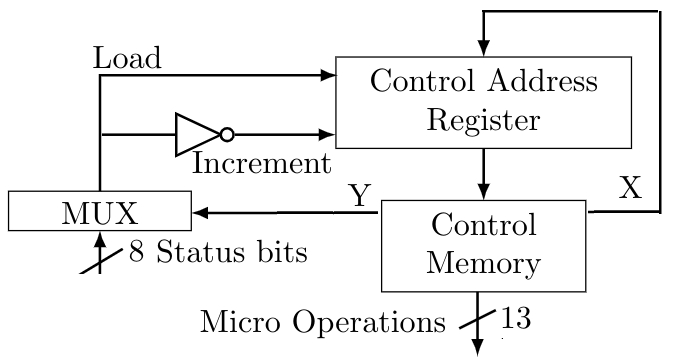
\includegraphics[scale=0.4]{./images/control_memory.jpeg} \end{center}\\ \hline
            \end{tabular} \end{myTableStyle} \vspace{0.08in}

  \begin{oneparchoices}
    \CorrectChoice  10, 3, 1024
    \choice         8, 5, 256
    \choice         5, 8, 2048
    \choice         10, 3, 512
  \end{oneparchoices}
  \\Hint: \quad X + Y + 13 = 26
  \\Hint: \quad Y = 3  \qquad 3 select bits are needed to select 8 i/p lines of MUX
  \\Hint: \quad X = 10 \qquad Size of Control memory = \( \mathbf { 2^{10} } \) Words
\end{questyle}
